
Bubble sort results:
From the plot we can see that the average running time on the unsorted data and the reverse order data both follow the same curve. Although the running time on the reverse sorted data is a little bit slower.
The average running time on the sorted data is way less and also follows a less steep curve.

\begin{figure}[H]
	\centering
	\begin{subfigure}[b]{0.5\textwidth}
		\centering
		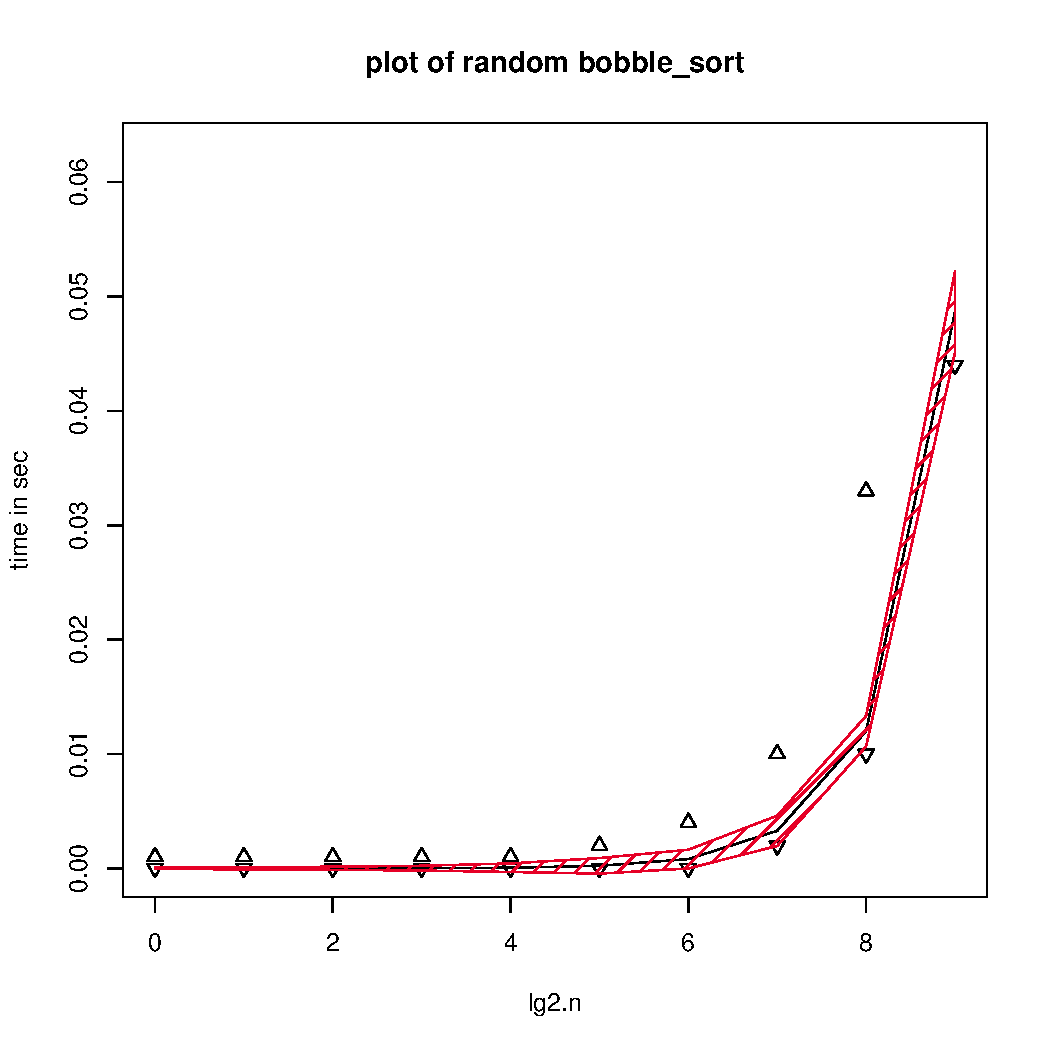
\includegraphics[width=\textwidth]{./pics/bobble_sort_random.pdf}
		\caption{bubble sort random input data}
	\end{subfigure}
	\hfill
	\begin{subfigure}[b]{0.5\textwidth}
		\centering
		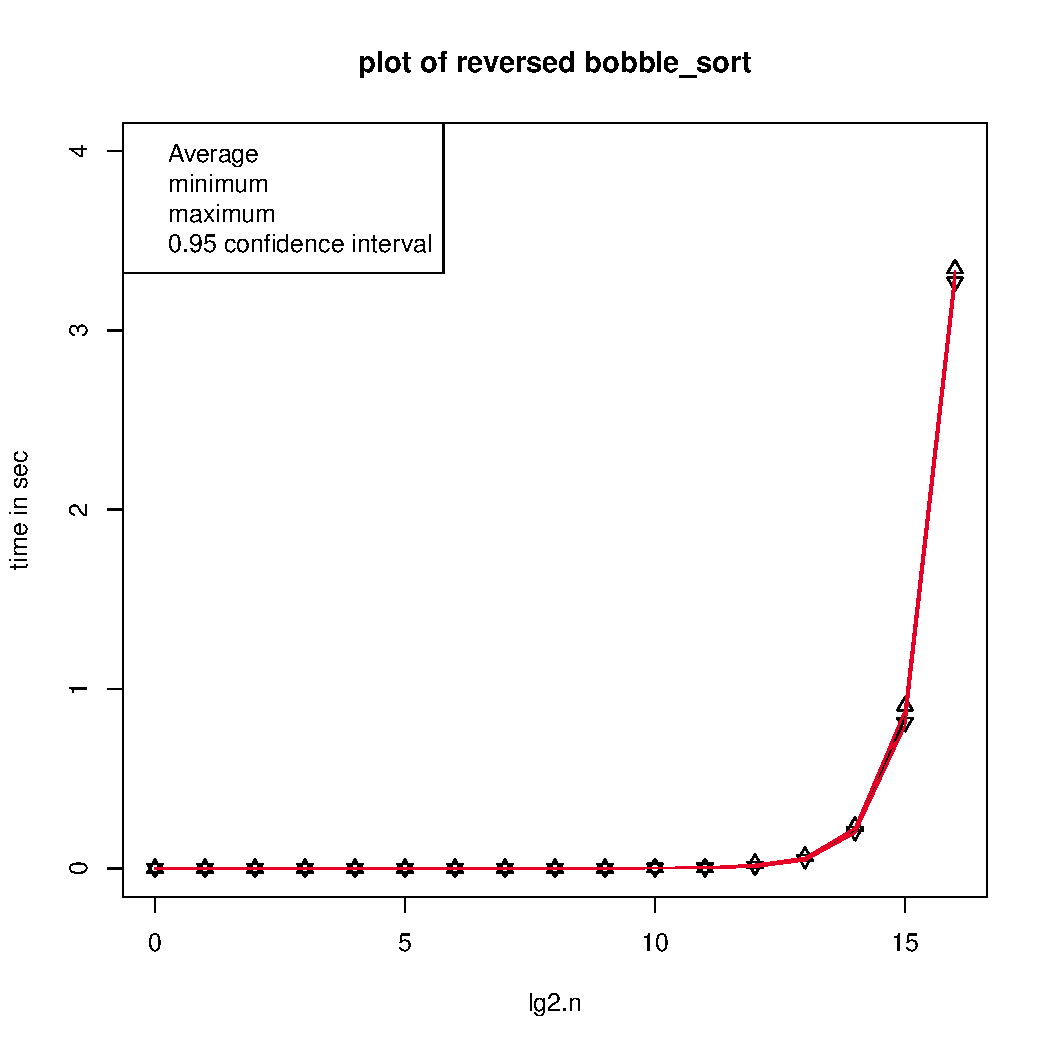
\includegraphics[width=\textwidth]{./pics/bobble_sort_reversed.pdf}
		\caption{bubble sort reversed sorted data}
	\end{subfigure}
	\hfill
	\begin{subfigure}[b]{0.5\textwidth}
		\centering
		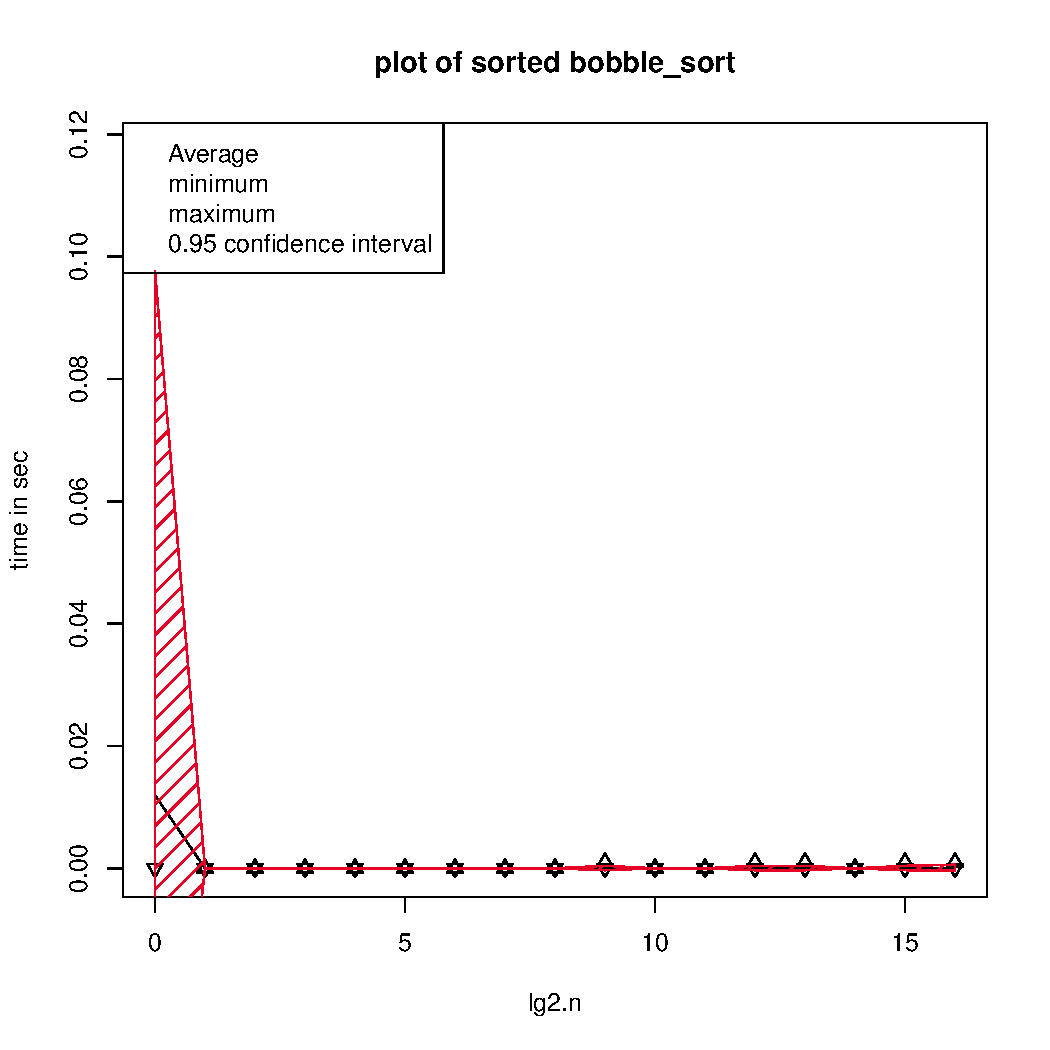
\includegraphics[width=\textwidth]{./pics/bobble_sort_sorted.pdf}
		\caption{bubble sort sorted data}
	\end{subfigure}
\end{figure}



Insertion sort results:
As we can se from the plots, the sorted order takes much way less time on average than the random order and reverse order.

\begin{figure}[H]
	\centering
	\begin{subfigure}[b]{0.5\textwidth}
		\centering
		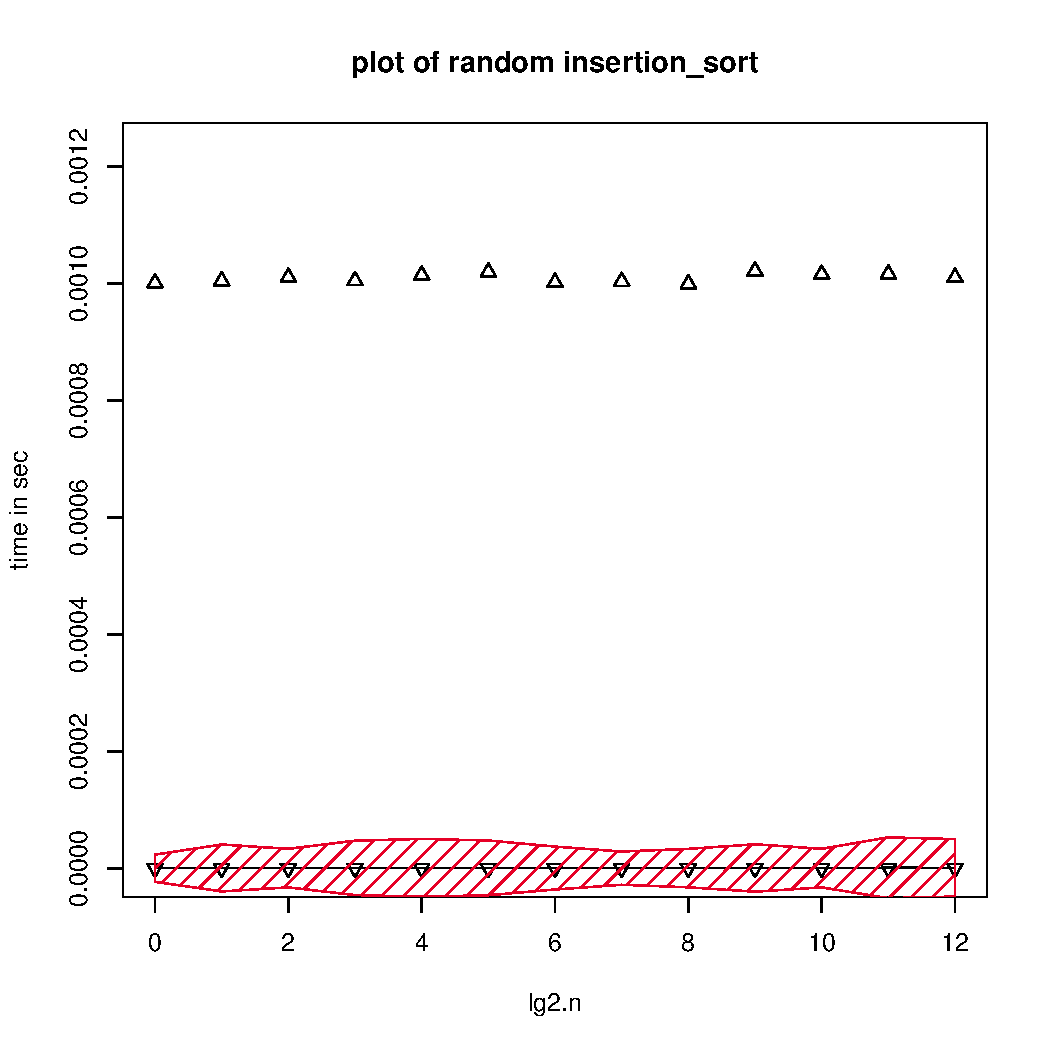
\includegraphics[width=\textwidth]{./pics/insertion_sort_random.pdf}
		\caption{Insertion sort random input data}
	\end{subfigure}
	\hfill
	\begin{subfigure}[b]{0.5\textwidth}
		\centering
		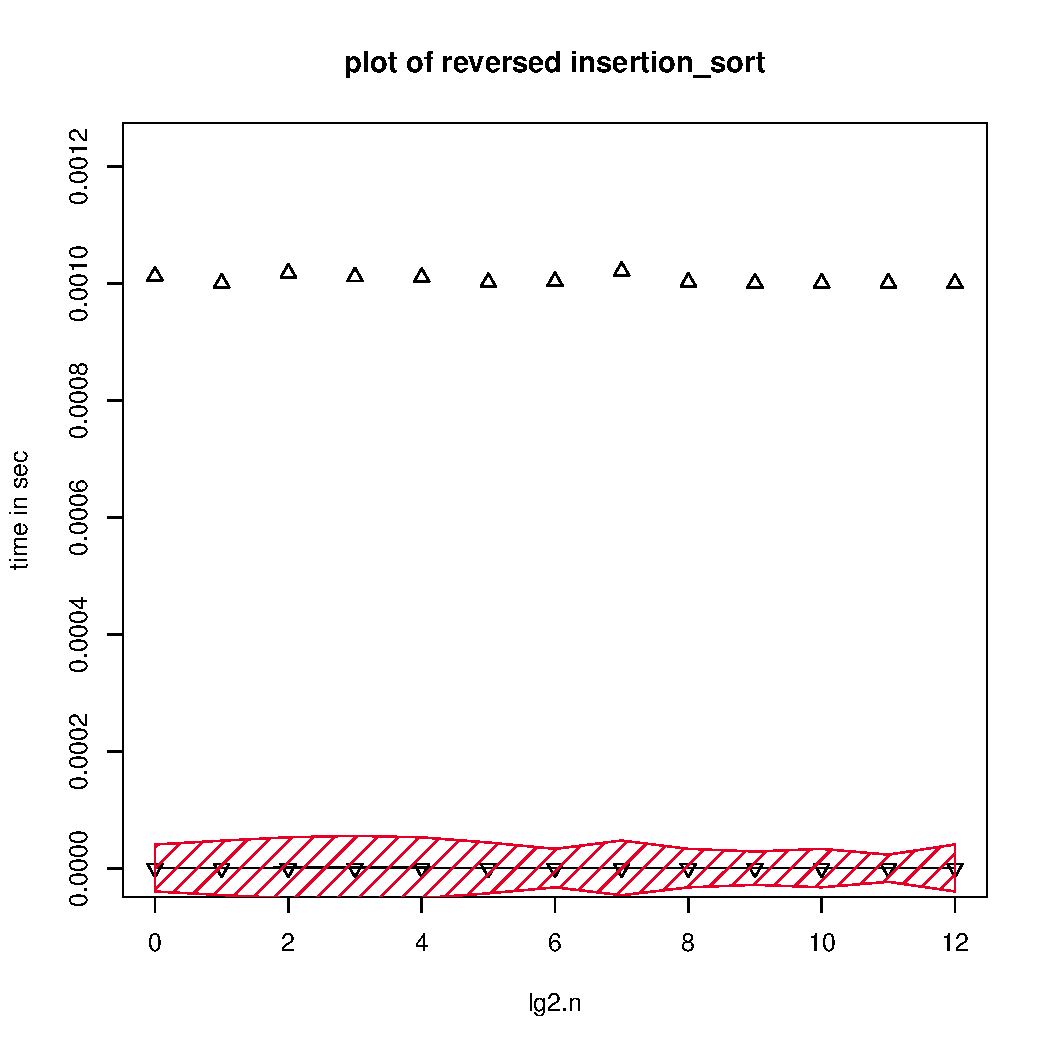
\includegraphics[width=\textwidth]{./pics/insertion_sort_reversed.pdf}
		\caption{Insertion sort reversed sorted data}
	\end{subfigure}
	\hfill
	\begin{subfigure}[b]{0.5\textwidth}
		\centering
		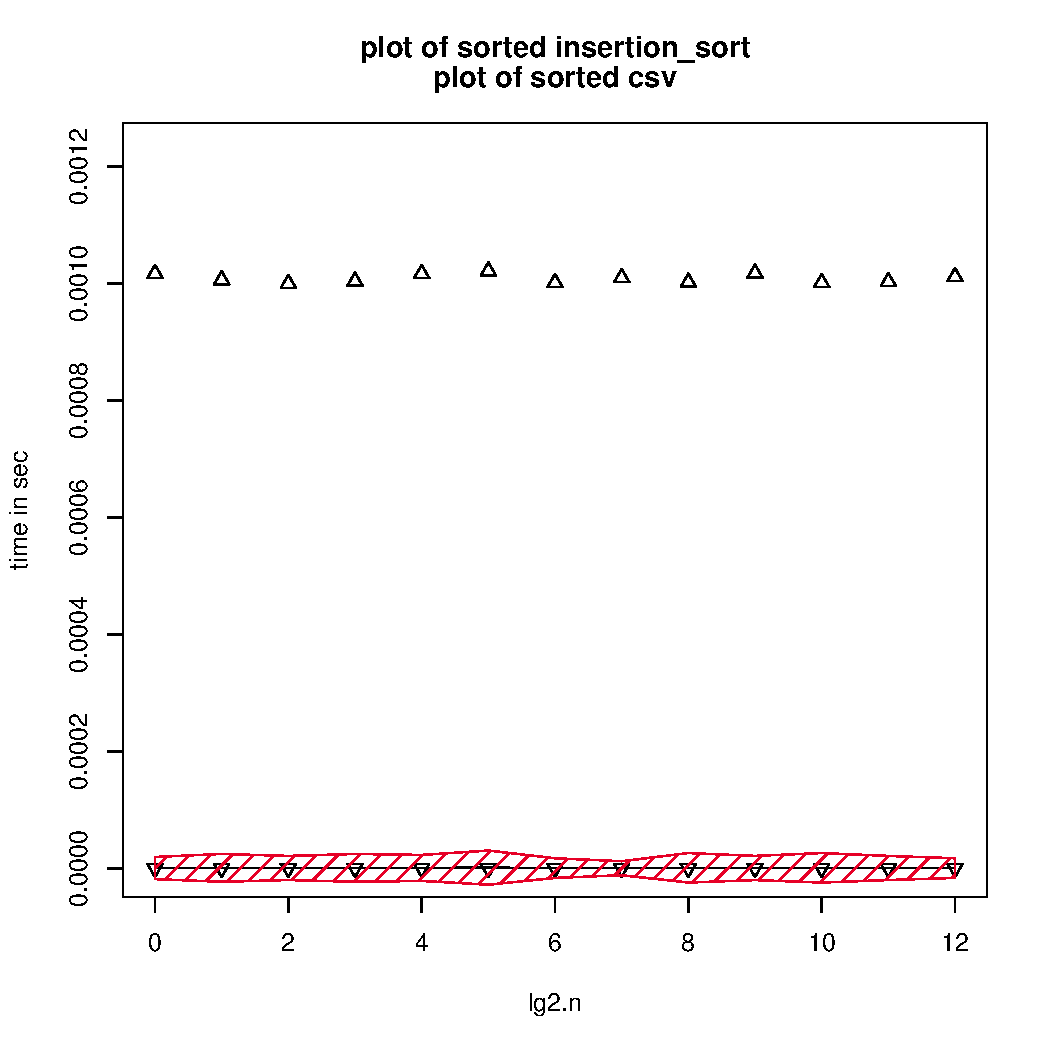
\includegraphics[width=\textwidth]{./pics/insertion_sort_sorted.pdf}
		\caption{Insertion sort sorted data}
	\end{subfigure}
\end{figure}

Quicksort results:
From the plot we can see that the average running time on sorted data and the reverse order data both follow the same curve. Although the running time on the sorted data is a little bit slower than the reverse sorted.
The average running time on the unsorted data is way less and also follows a less steep curve.


\begin{figure}[H]
	\centering
	\begin{subfigure}[b]{0.5\textwidth}
		\centering
		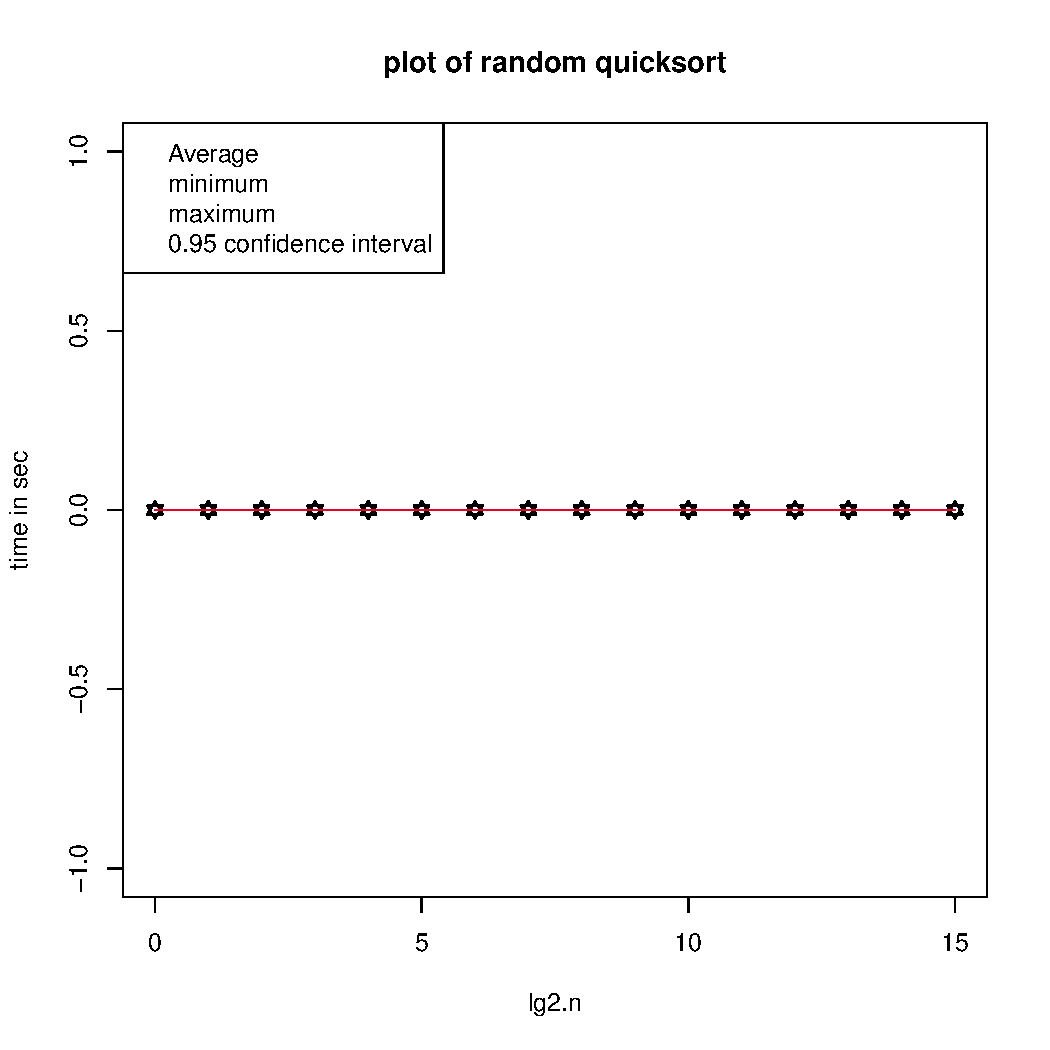
\includegraphics[width=\textwidth]{./pics/quicksort_random.pdf}
		\caption{Quicksort random input data}
	\end{subfigure}
	\hfill
	\begin{subfigure}[b]{0.5\textwidth}
		\centering
		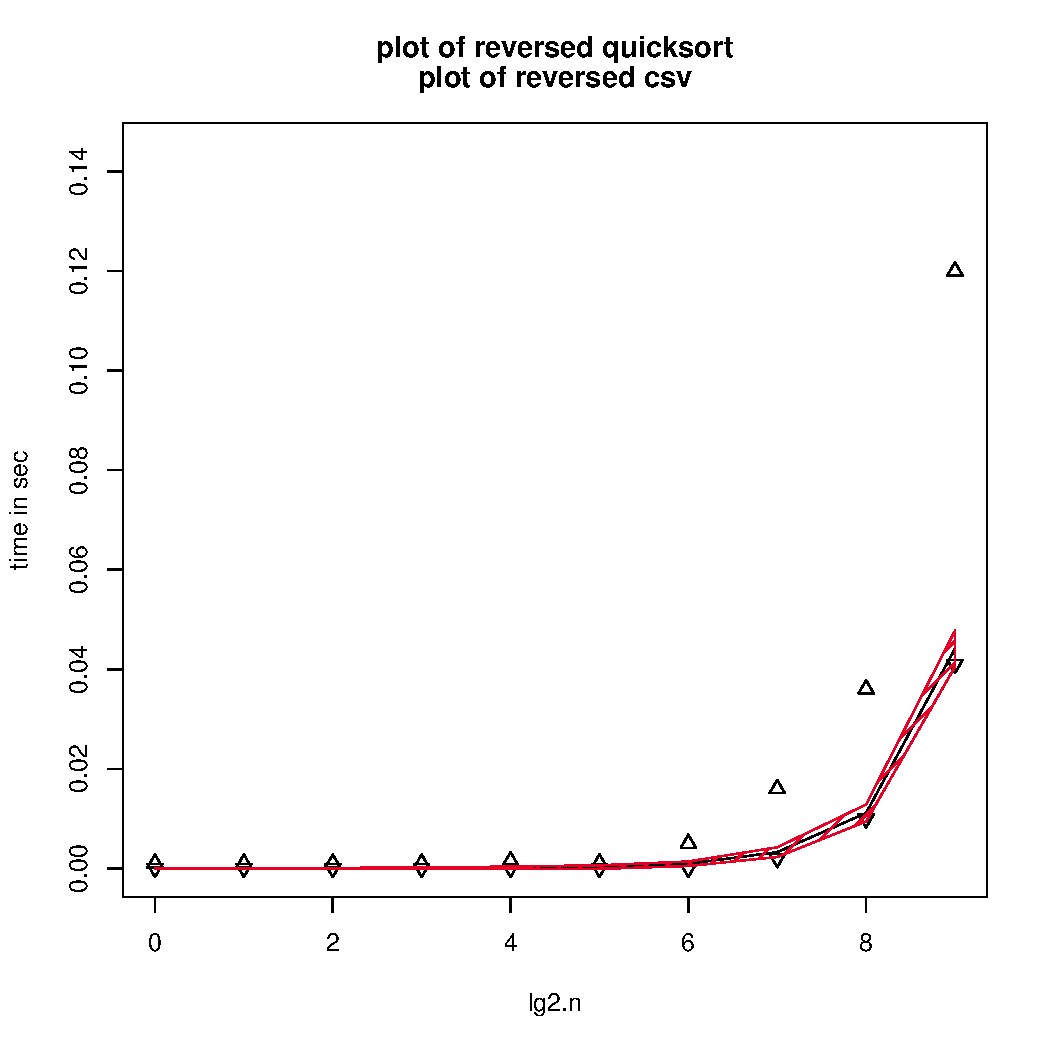
\includegraphics[width=\textwidth]{./pics/quicksort_reversed.pdf}
		\caption{Quicksort reversed sorted data}
	\end{subfigure}
	\hfill
	\begin{subfigure}[b]{0.5\textwidth}
		\centering
		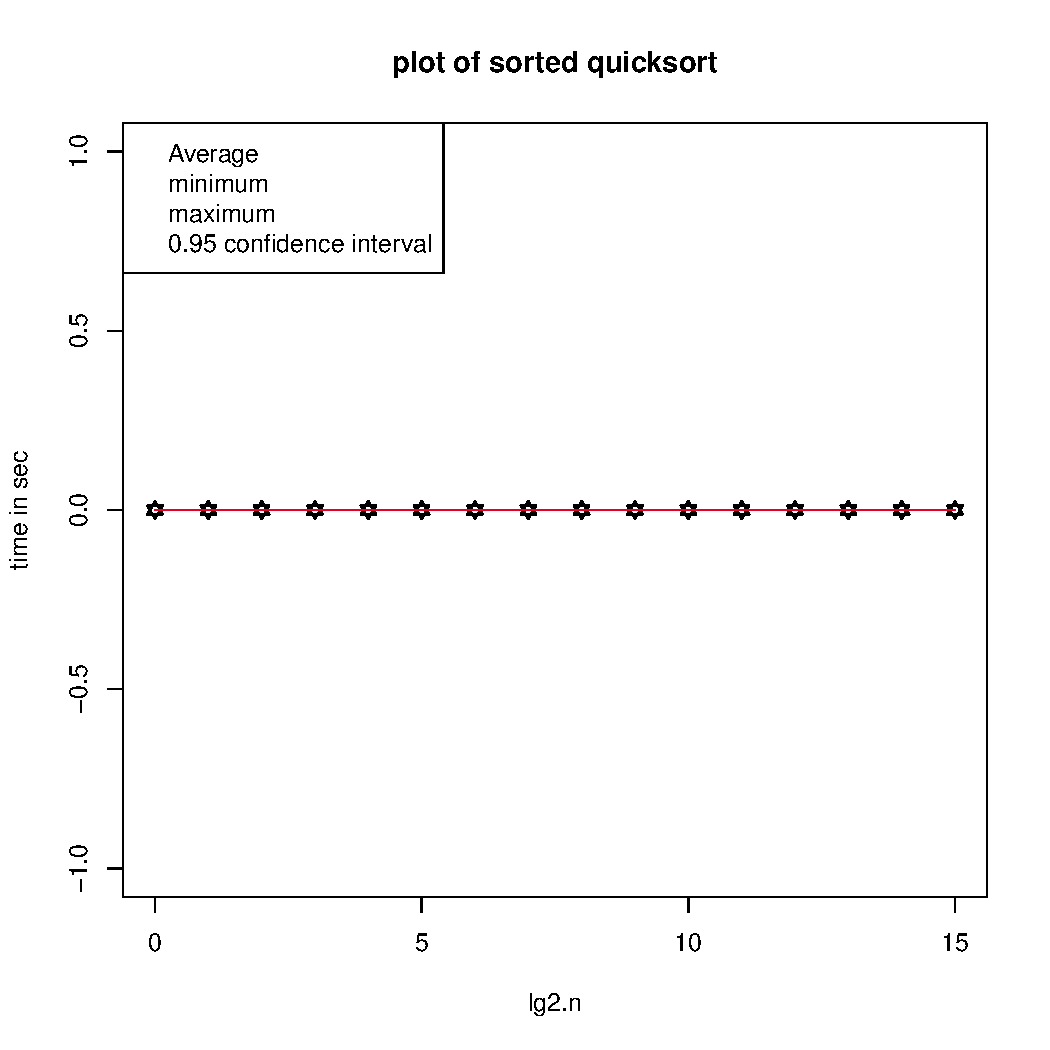
\includegraphics[width=\textwidth]{./pics/quicksort_sorted.pdf}
		\caption{Quicksort sorted data}
	\end{subfigure}
\end{figure}

Quicksort Insertion sort hybrid results:
The Quicksort insertion sort hybrid outperformes both quicksort and insertionsort on the unsorted data and the reverse sorted data. In fact, on the unsorted data, it is the best performing algorithm of all tested. On the sorted data it is beaten by insertionsort though.

\begin{figure}[H]
	\centering
	\begin{subfigure}[b]{0.5\textwidth}
		\centering
		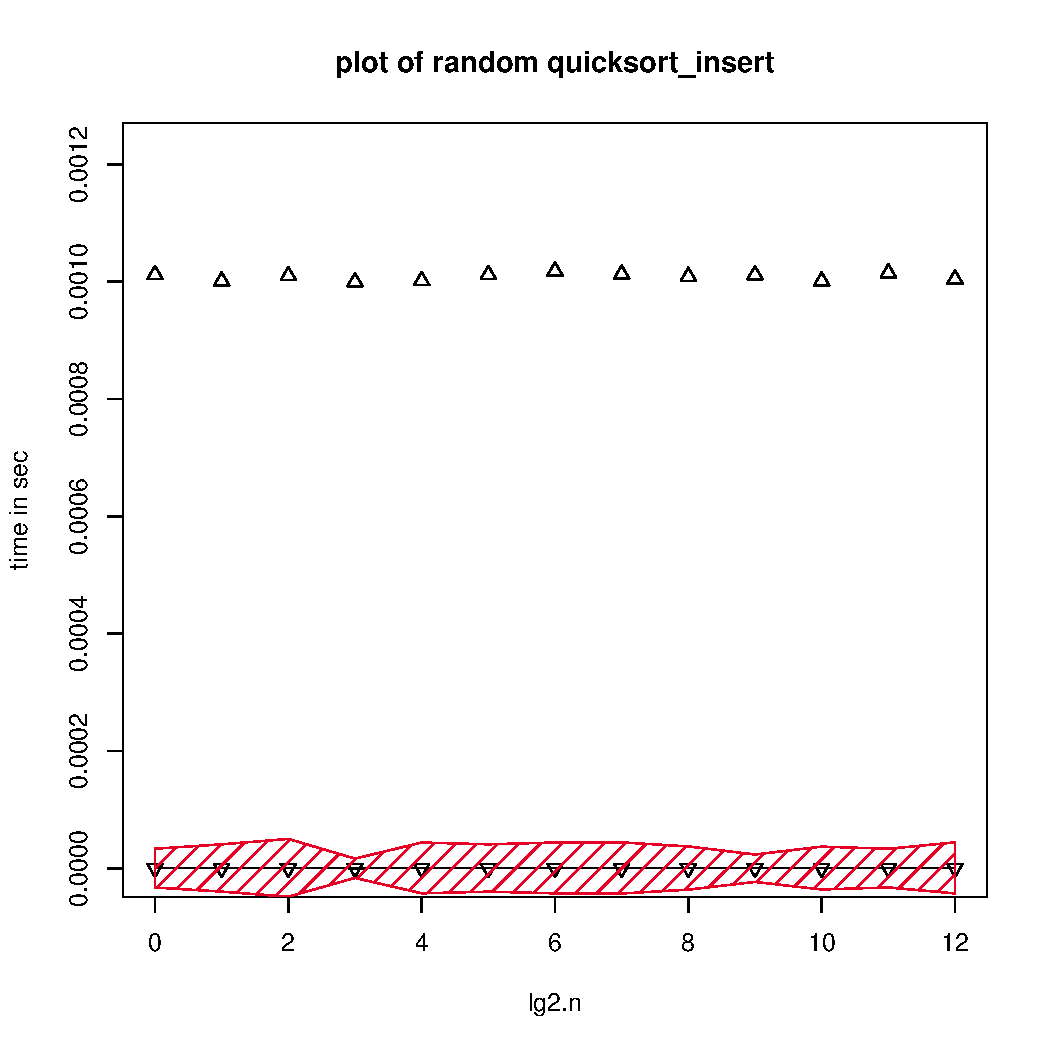
\includegraphics[width=\textwidth]{./pics/quicksort_insert_random.pdf}
		\caption{Quicksort Insertion sort random input data}
	\end{subfigure}
	\hfill
	\begin{subfigure}[b]{0.5\textwidth}
		\centering
		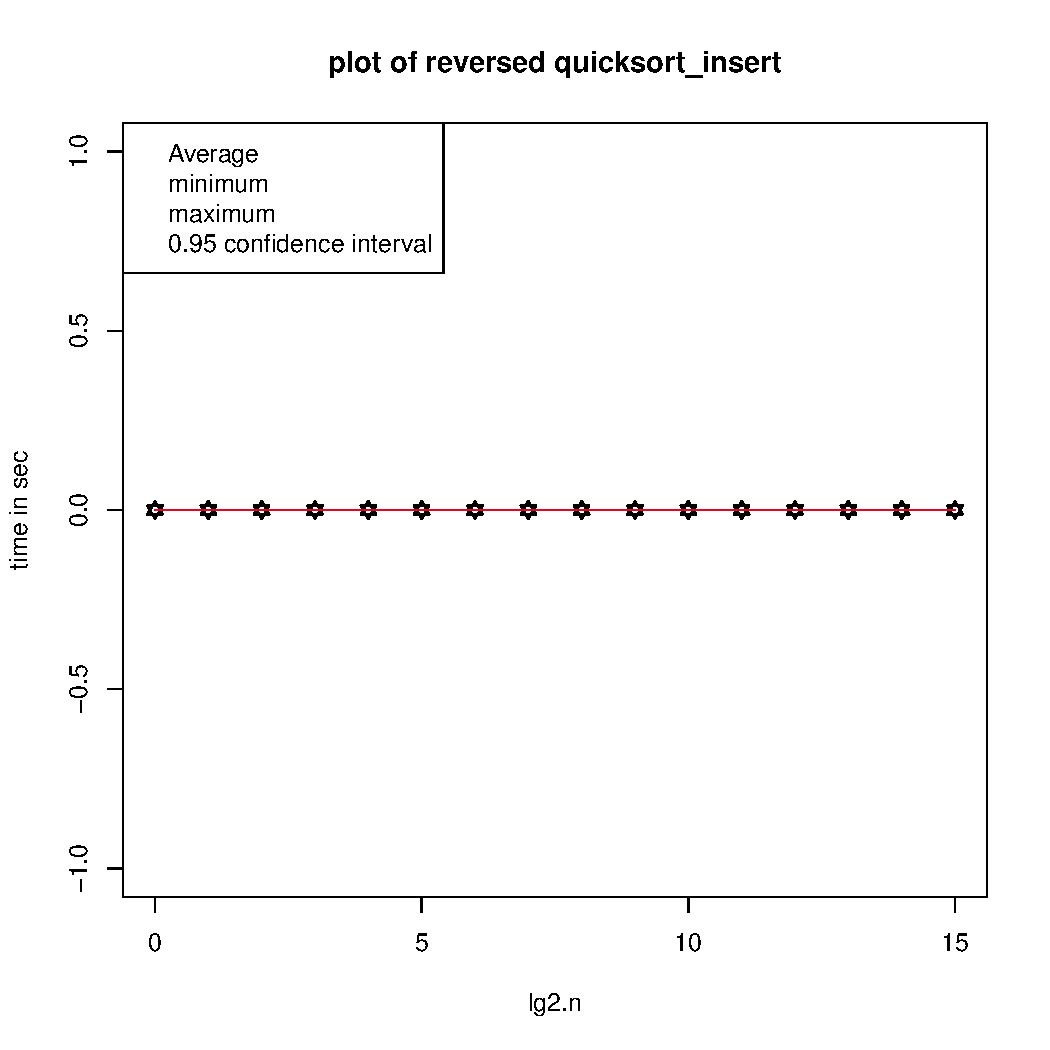
\includegraphics[width=\textwidth]{./pics/quicksort_insert_reversed.pdf}
		\caption{Quicksort Insertion sort reversed sorted data}
	\end{subfigure}
	\hfill
	\begin{subfigure}[b]{0.5\textwidth}
		\centering
		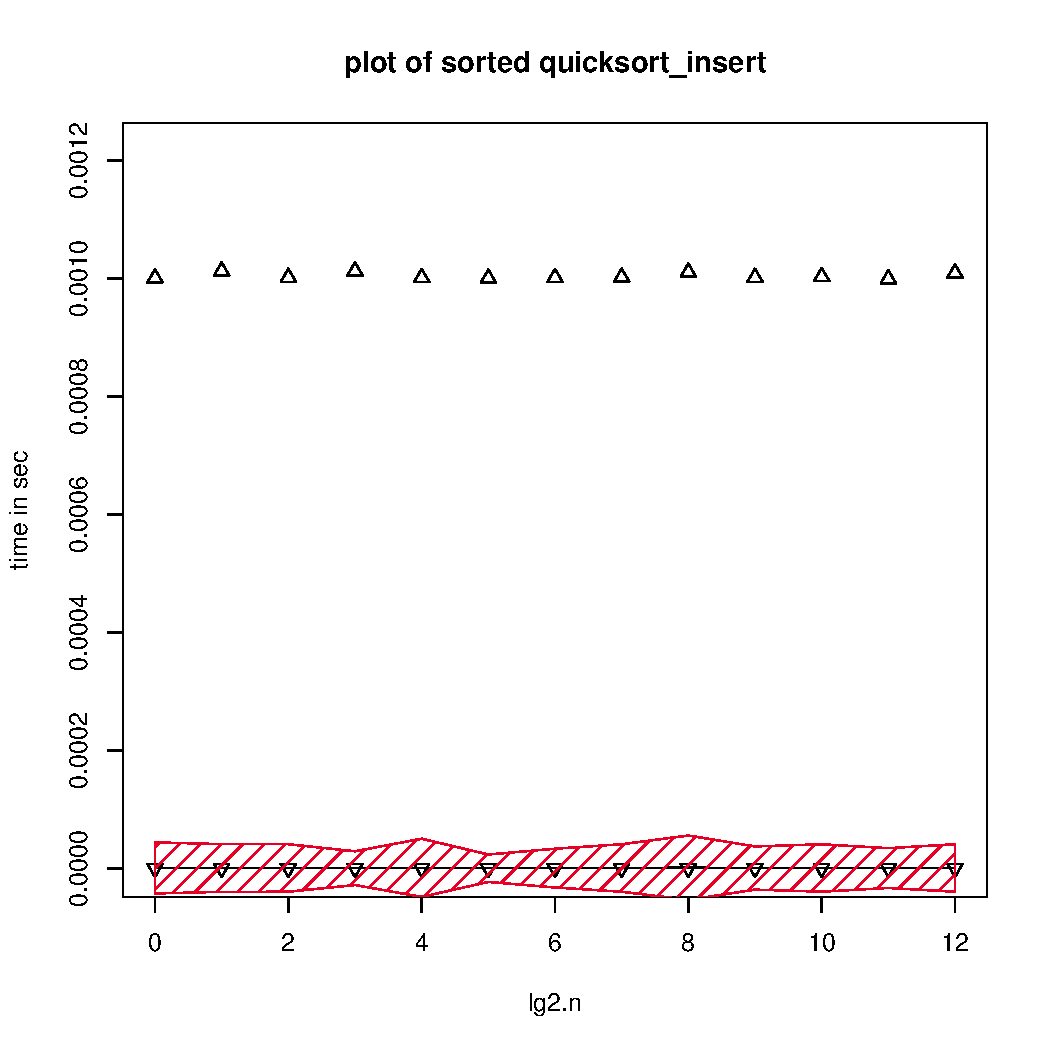
\includegraphics[width=\textwidth]{./pics/quicksort_insert_sorted.pdf}
		\caption{Quicksort Insertion sort sorted data}
	\end{subfigure}
\end{figure}


Mergesort results:
Both the unsorted data, the sorted and the reverse sorted follows the same curve for the average running time. The unsorted data hade the shortest running time, followed by the reverse ordered and the ordered data.

\begin{figure}[H]
	\centering
	\begin{subfigure}[b]{0.5\textwidth}
		\centering
		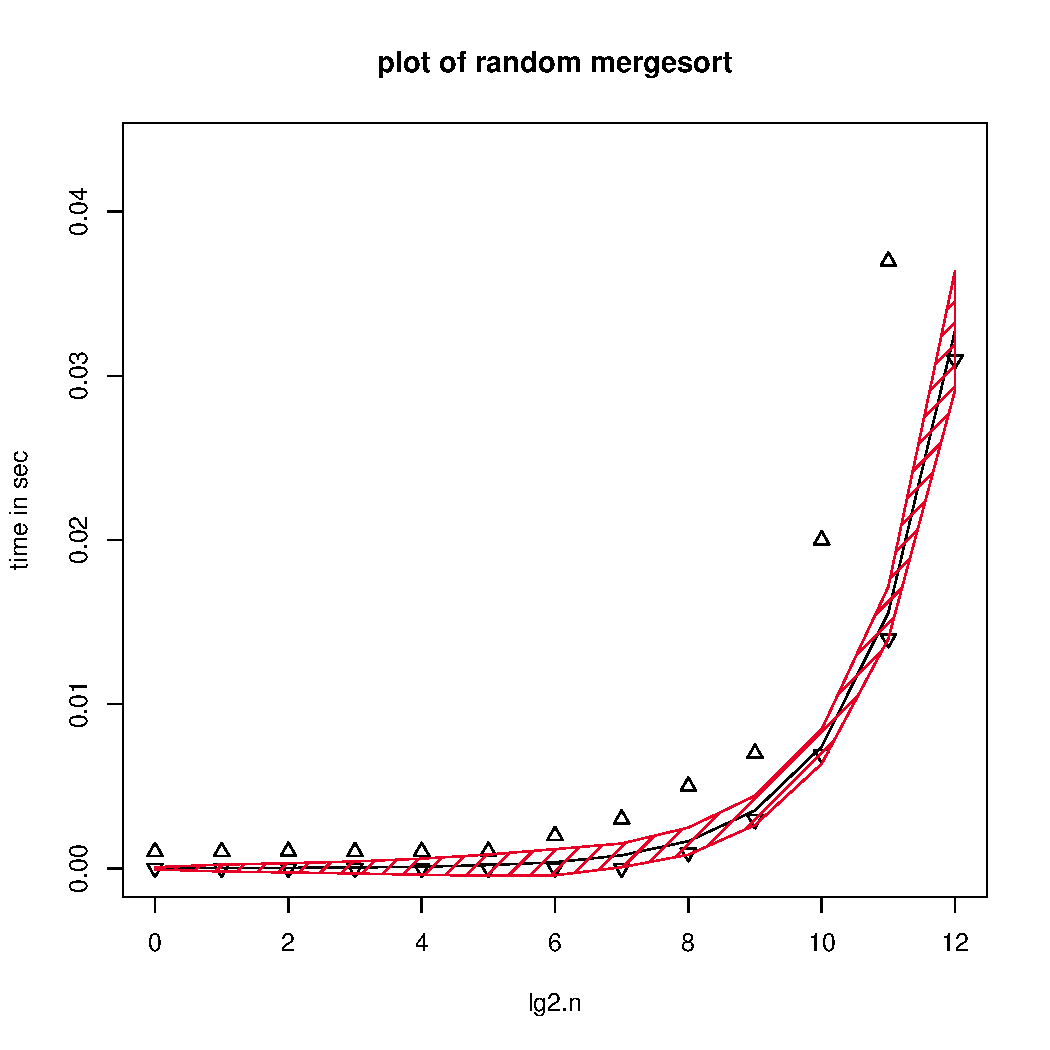
\includegraphics[width=\textwidth]{./pics/mergesort_random.pdf}
		\caption{mergesort random input data}
	\end{subfigure}
	\hfill
	\begin{subfigure}[b]{0.5\textwidth}
		\centering
		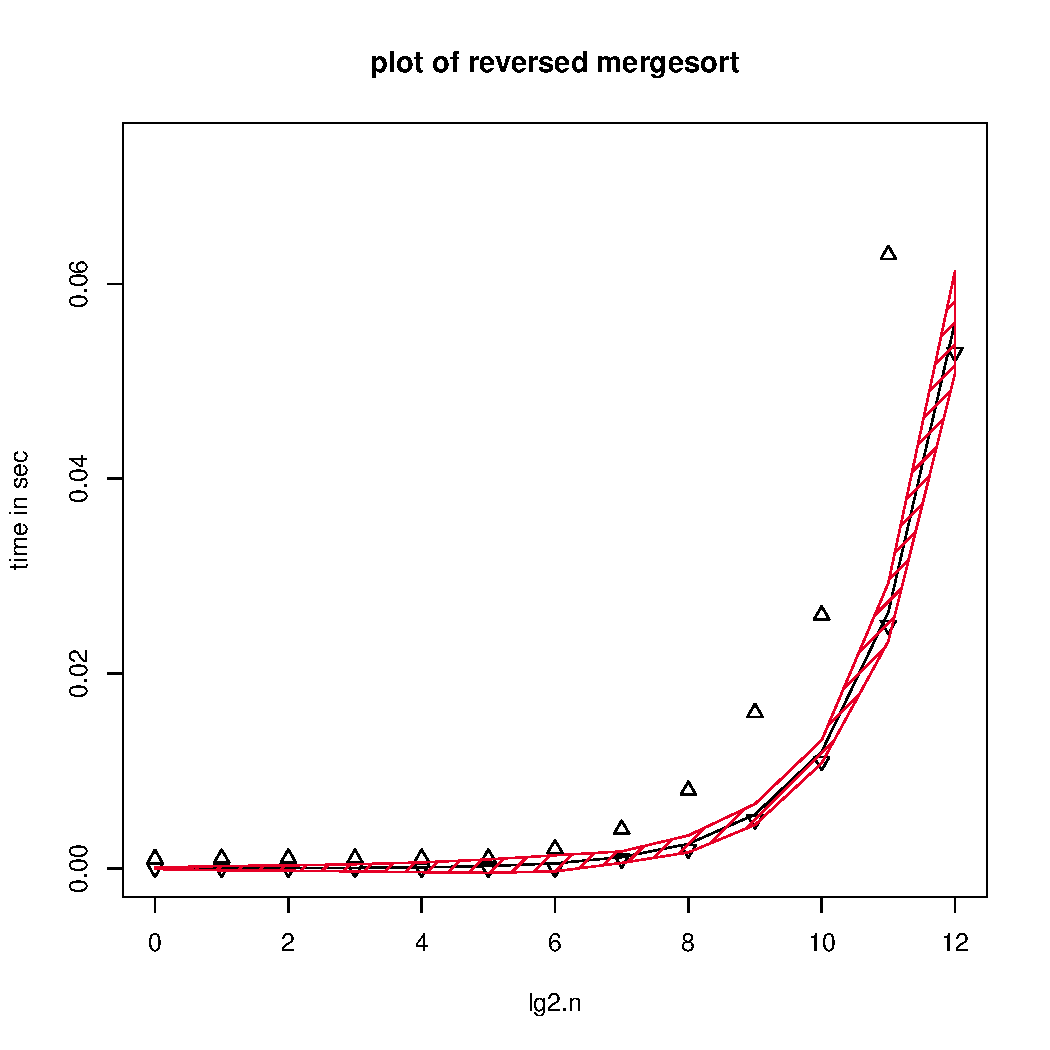
\includegraphics[width=\textwidth]{./pics/mergesort_reversed.pdf}
		\caption{mergesort reversed sorted data}
	\end{subfigure}
	\hfill
	\begin{subfigure}[b]{0.5\textwidth}
		\centering
		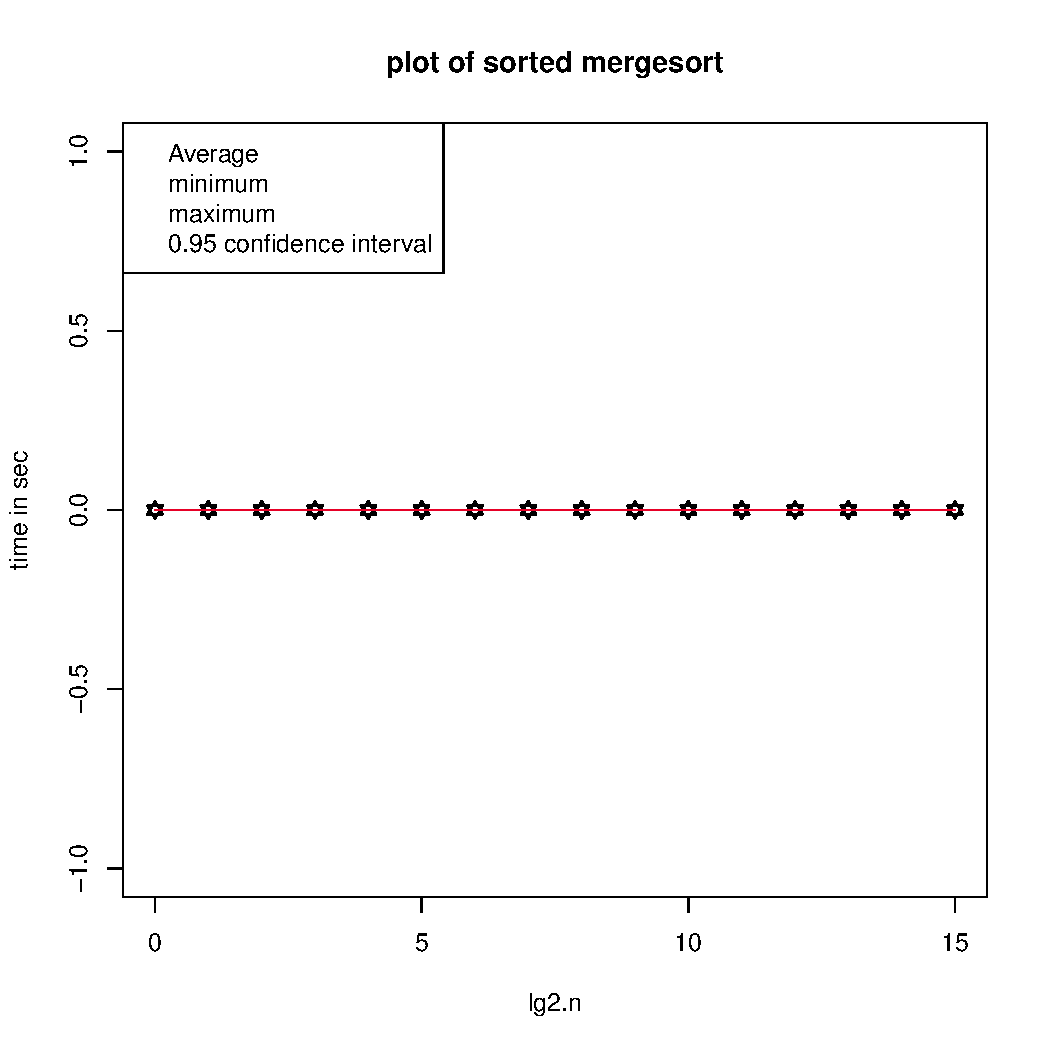
\includegraphics[width=\textwidth]{./pics/mergesort_sorted.pdf}
		\caption{mergesort sorted data}
	\end{subfigure}
\end{figure}

Mergesort Insertion sort hybrid results:
The mergesort insertionsort hybrid outperformed mergesort slightly on the unsorted data and significantly on the reverse sorted data. It took way longer time than insertionsort though.

\begin{figure}[H]
	\centering
	\begin{subfigure}[b]{0.5\textwidth}
		\centering
		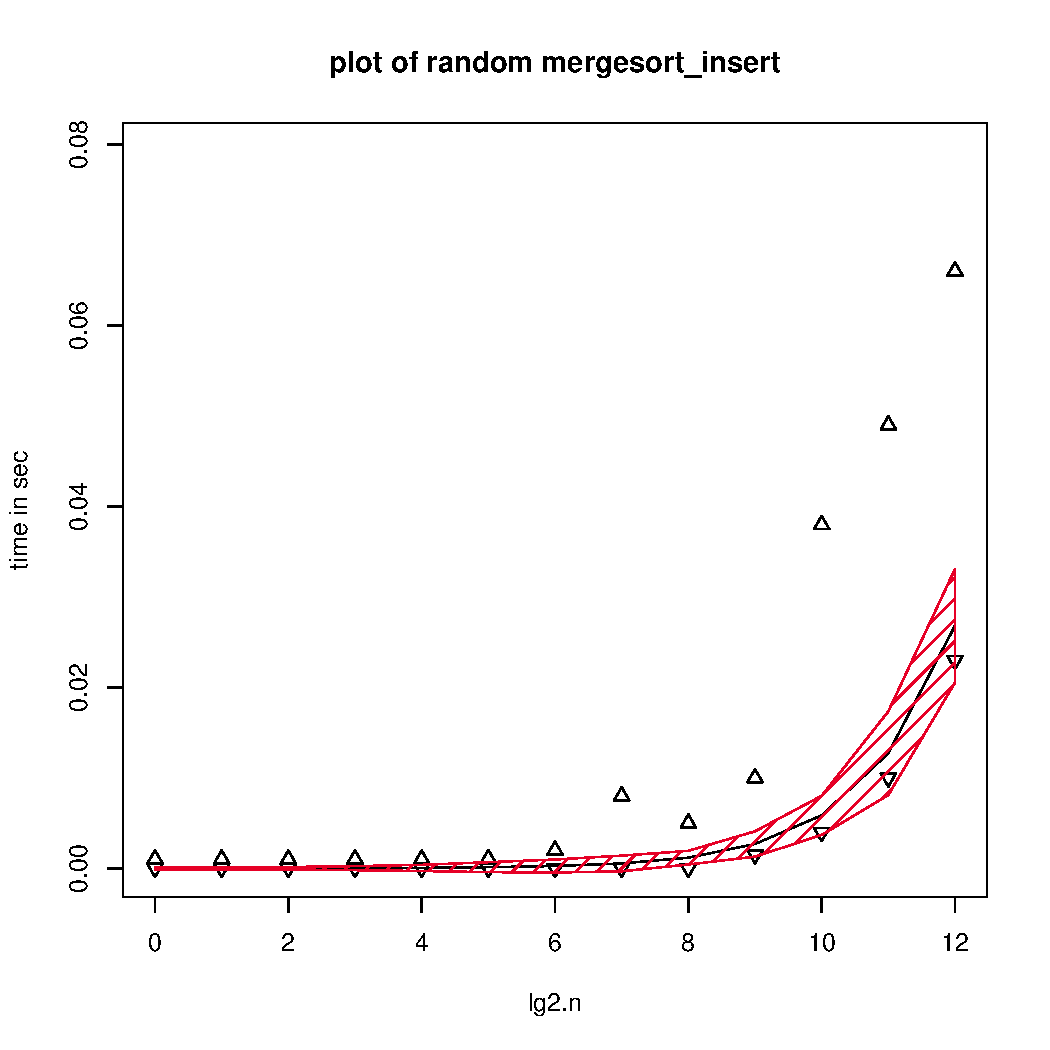
\includegraphics[width=\textwidth]{./pics/mergesort_insert_random.pdf}
		\caption{Mergesort Insertion sort random input data}
	\end{subfigure}
	\hfill
	\begin{subfigure}[b]{0.5\textwidth}
		\centering
		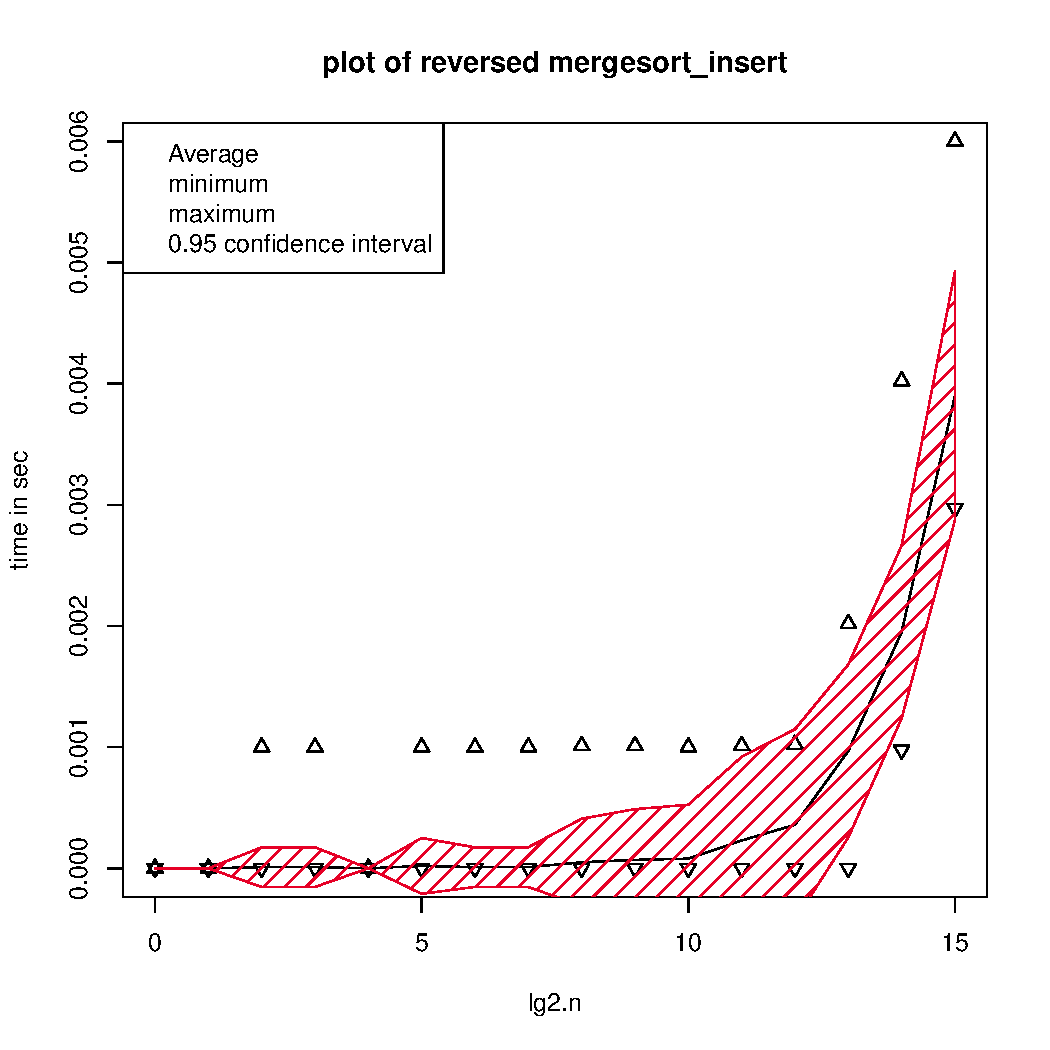
\includegraphics[width=\textwidth]{./pics/mergesort_insert_reversed.pdf}
		\caption{Mergesort Insertion sort reversed sorted data}
	\end{subfigure}
	\hfill
	\begin{subfigure}[b]{0.5\textwidth}
		\centering
		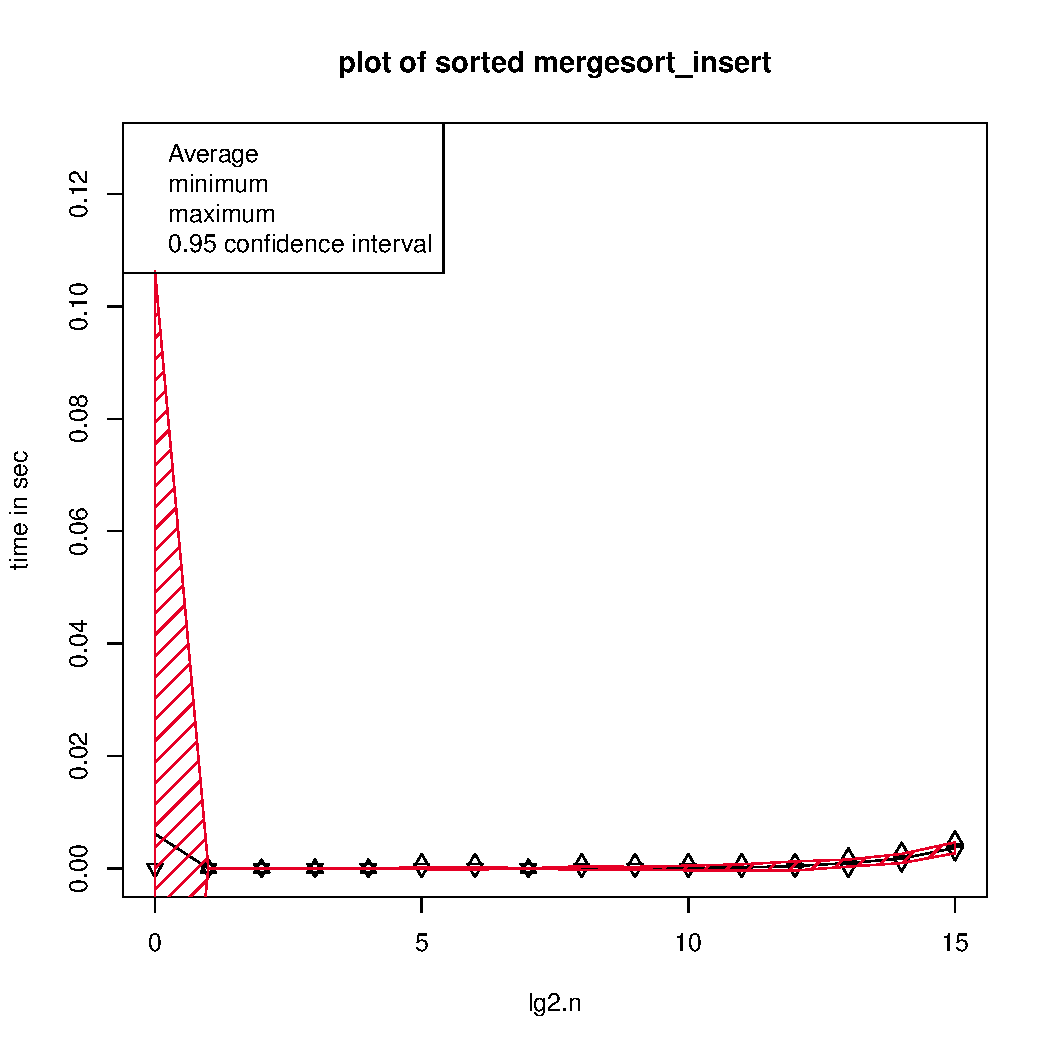
\includegraphics[width=\textwidth]{./pics/mergesort_insert_sorted.pdf}
		\caption{Mergesort Insertion sort sorted data}
	\end{subfigure}
\end{figure}

Python sort results:
Pythonsort is the best performing algorithm on the reverse sorted data, of all tested.

\begin{figure}[H]
	\centering
	\begin{subfigure}[b]{0.5\textwidth}
		\centering
		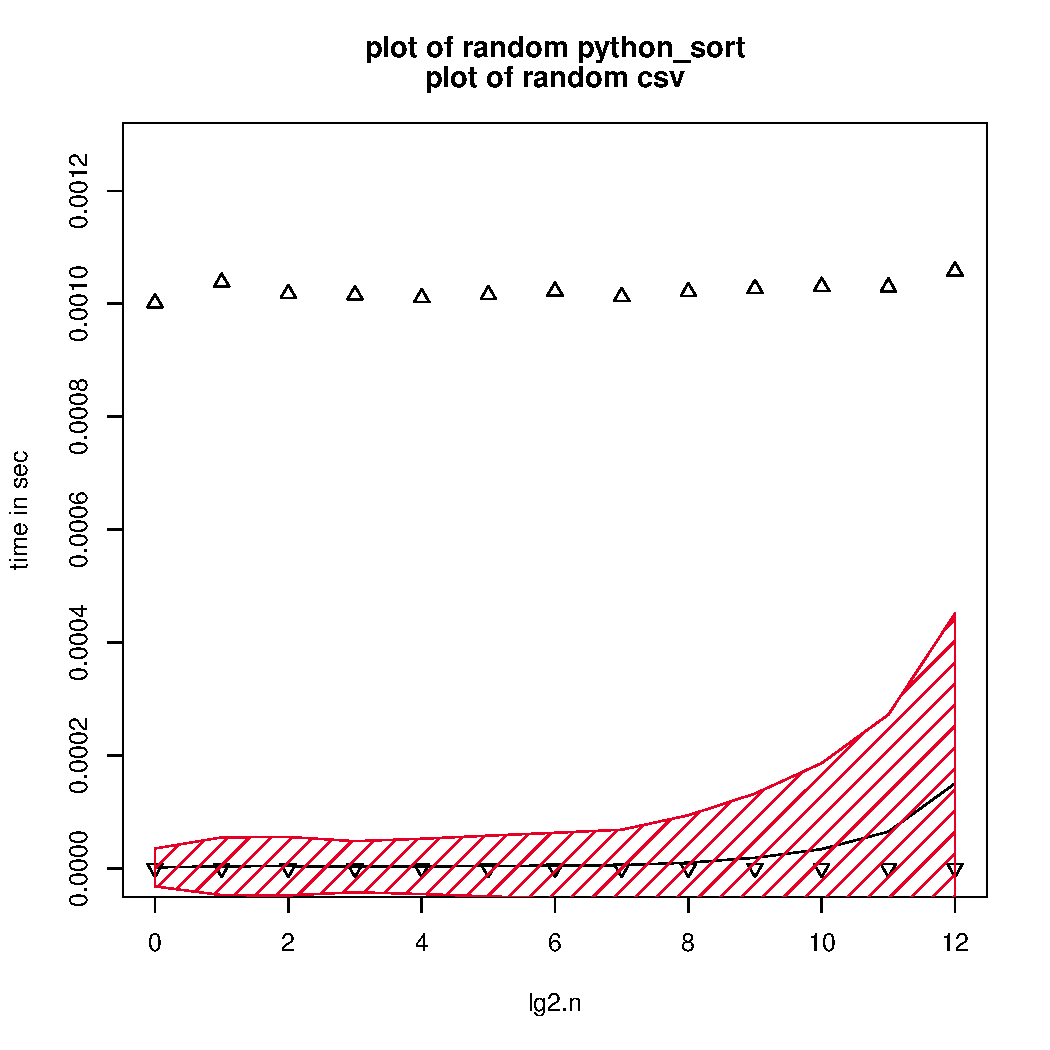
\includegraphics[width=\textwidth]{./pics/python_sort_random.pdf}
		\caption{python sort random input data}
	\end{subfigure}
	\hfill
	\begin{subfigure}[b]{0.5\textwidth}
		\centering
		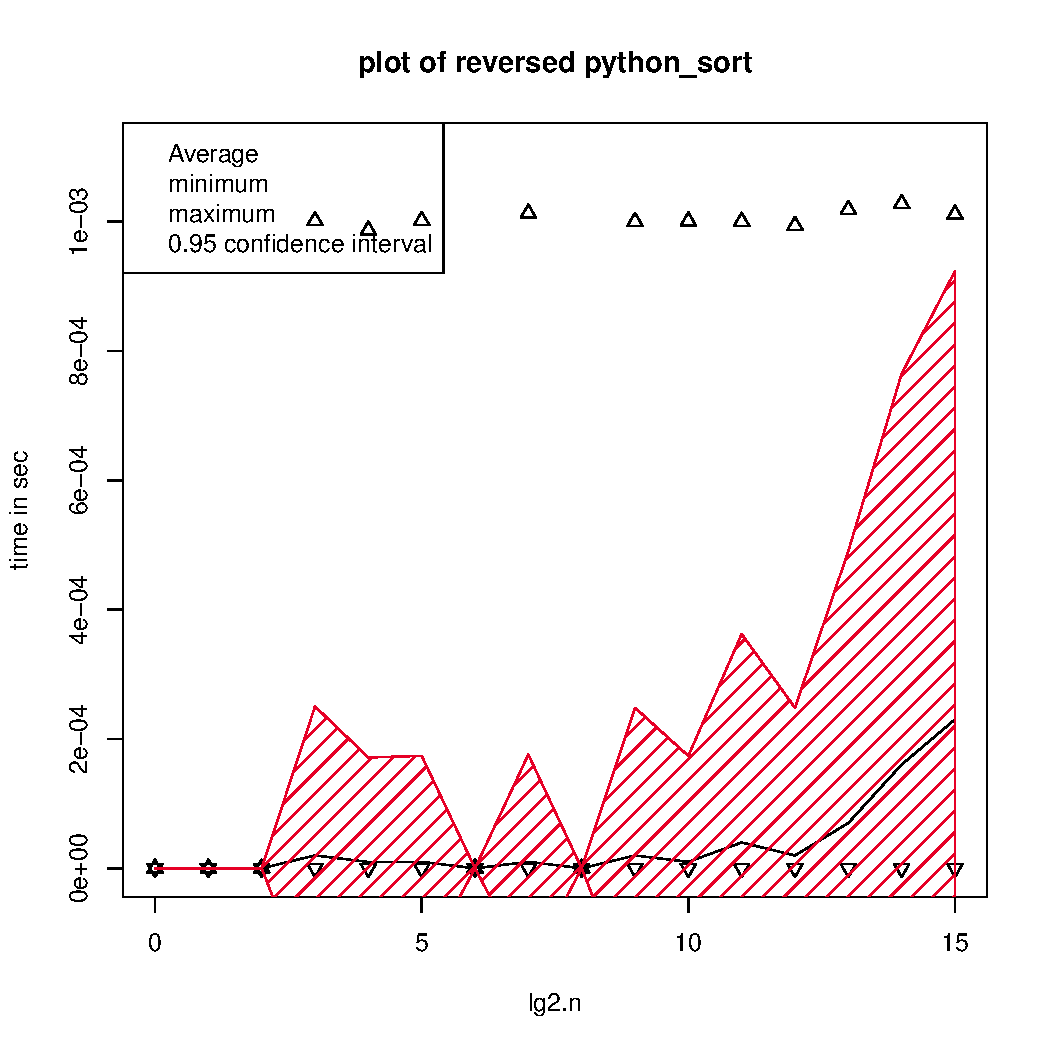
\includegraphics[width=\textwidth]{./pics/python_sort_reversed.pdf}
		\caption{python sort reversed sorted data}
	\end{subfigure}
	\hfill
	\begin{subfigure}[b]{0.5\textwidth}
		\centering
		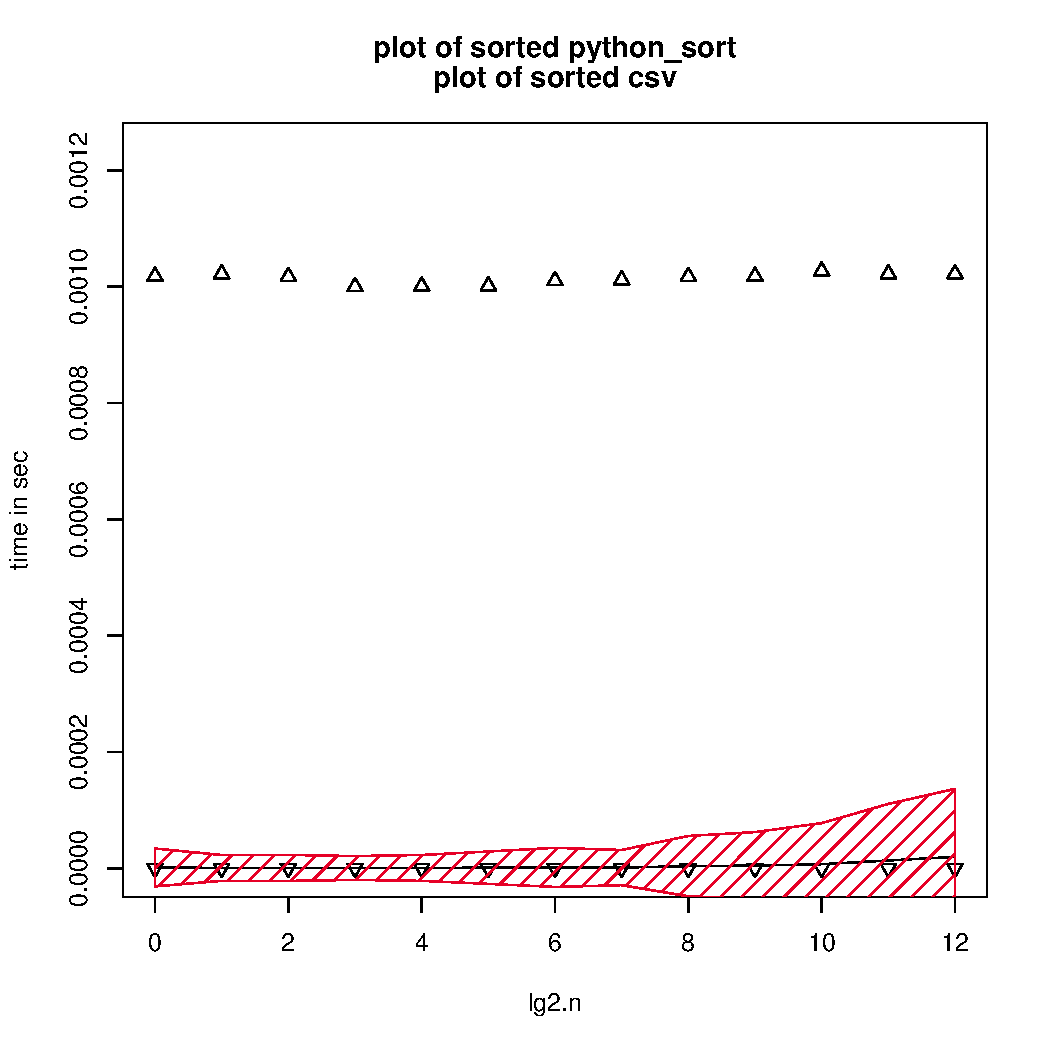
\includegraphics[width=\textwidth]{./pics/python_sort_sorted.pdf}
		\caption{python sort sorted data}
	\end{subfigure}
\end{figure}


Numpy sort results:

\begin{figure}[H]
	\centering
	\begin{subfigure}[b]{0.5\textwidth}
		\centering
		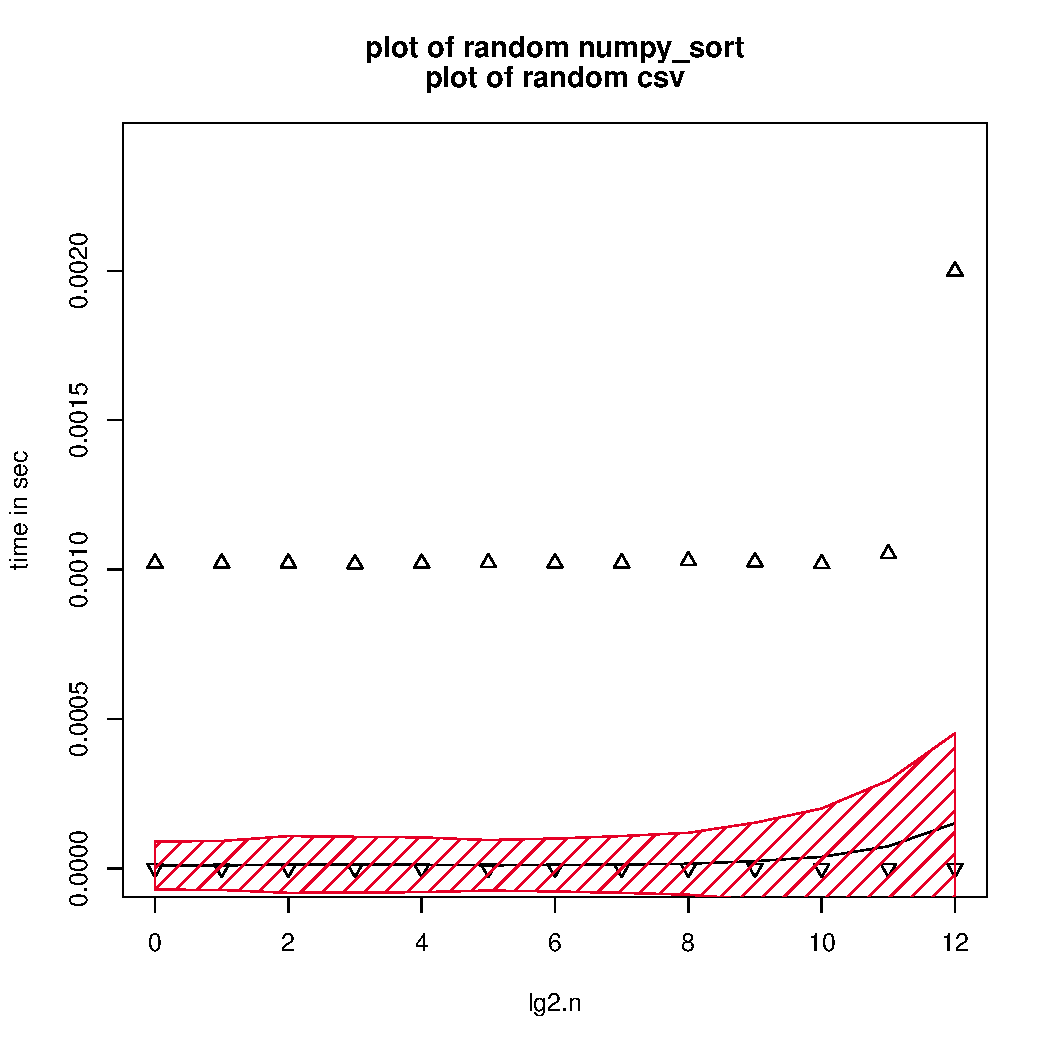
\includegraphics[width=\textwidth]{./pics/numpy_sort_random.pdf}
		\caption{numpy sort random input data}
	\end{subfigure}
	\hfill
	\begin{subfigure}[b]{0.5\textwidth}
		\centering
		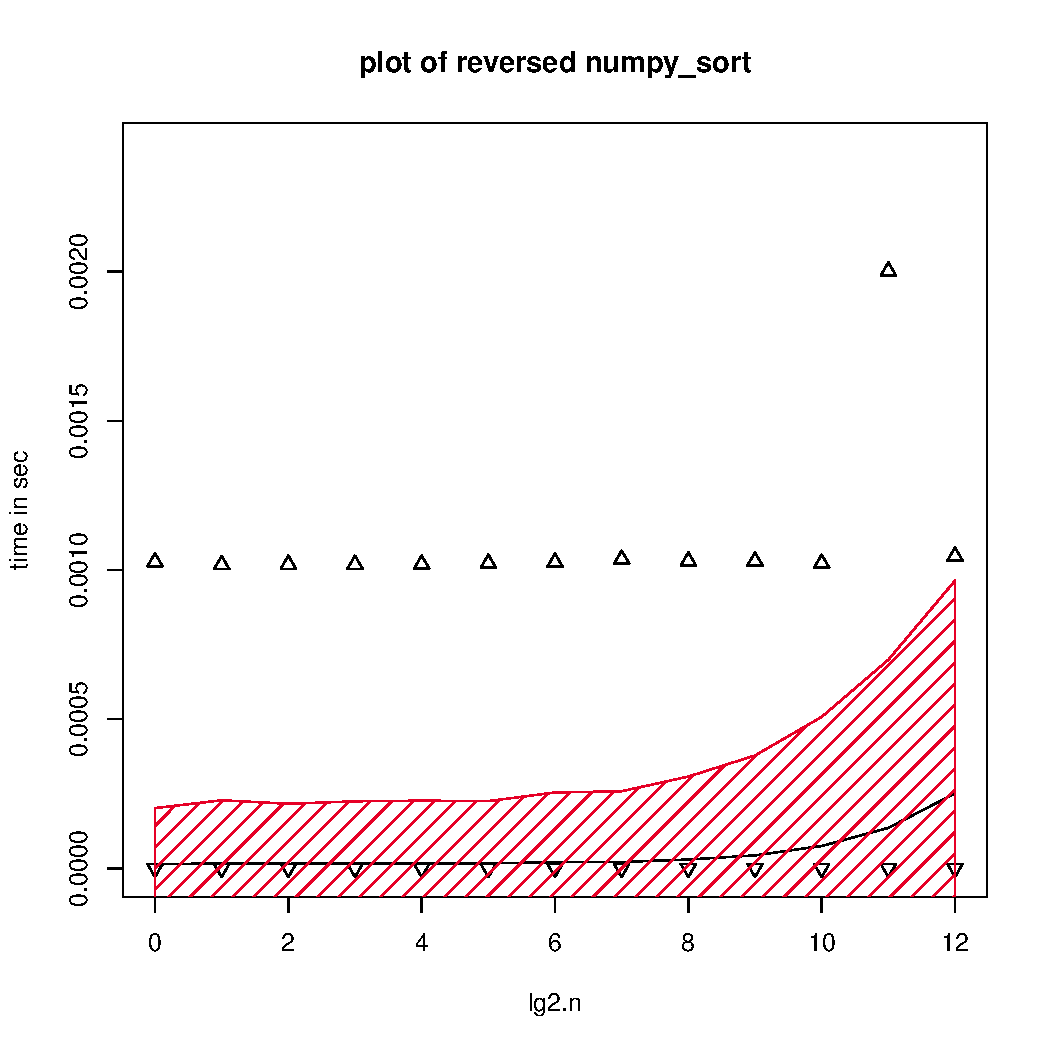
\includegraphics[width=\textwidth]{./pics/numpy_sort_reversed.pdf}
		\caption{numpy sort reversed sorted data}
	\end{subfigure}
	\hfill
	\begin{subfigure}[b]{0.5\textwidth}
		\centering
		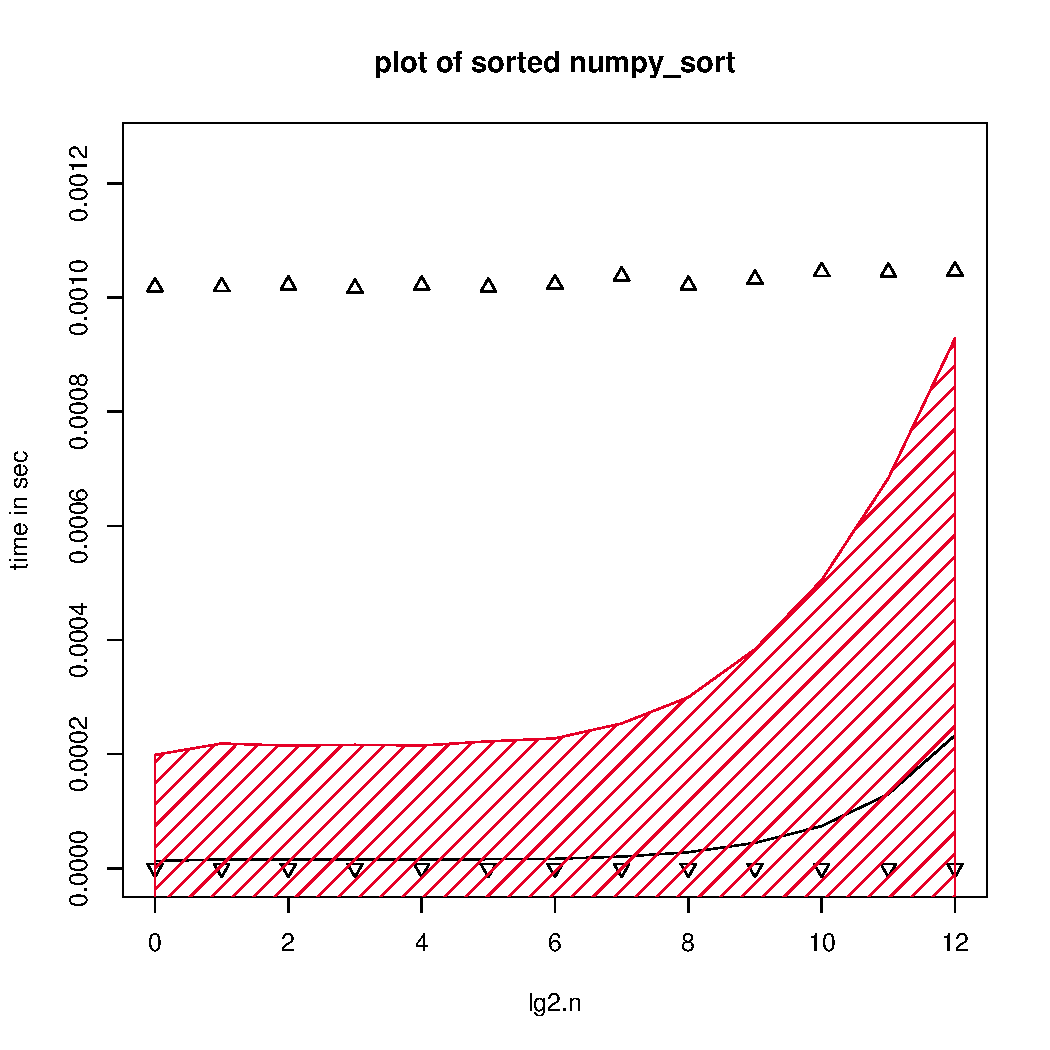
\includegraphics[width=\textwidth]{./pics/numpy_sort_sorted.pdf}
		\caption{numpy sort sorted data}
	\end{subfigure}
\end{figure}
